\documentclass{COMPXXXX}
\usepackage{times}
\usepackage{graphicx}
\usepackage{latexsym}
\usepackage{amssymb}
\usepackage{listings}
\usepackage{algorithm,algpseudocode}
\usepackage{amsmath}
\usepackage{hyperref}
\usepackage{amsthm}
\usepackage{booktabs}
\usepackage{subcaption}

\begin{document}

\title{Explainable Ensemble Learning and Symbolic Baseline Benchmarking for Retail Loan Approval Prediction}

\author{Kirtan Karkar\institute{School of Computing and Mathematical Sciences, University of Greenwich, London SE10 9LS, UK, email: kirtan.karkar@gre.ac.uk}}

\maketitle
\bibliographystyle{COMPXXXX}

\begin{abstract}
Automated credit appraisal systems balance institutional default risk against fair consumer access to credit. This study adapts and critically evaluates the explainable Random Forest--XGBoost soft-voting framework of Gawande et al.~\cite{gawande2026} on the canonical Kaggle Loan Prediction dataset ($N=614$, 11 predictors), contrasting trivial baselines, symbolic rule engines, and tuned statistical classifiers under leak-free nested stratified $5\times 3$ cross-validation optimizing Macro F1. Contrary to claims on large corporate benchmarks ($N > 10^4$), complex ensembles do not yield significant gains over simpler interpretable models at modest sample sizes: the RF--XGBoost soft-voting ensemble achieves Test Accuracy $=0.837$ and Test Macro F1 $=0.784$ (Nested CV $=0.692 \pm 0.083$), whereas Logistic Regression reaches $0.862$ accuracy ($0.815$ Macro F1; CV $=0.711 \pm 0.089$), and a one-rule credit-history heuristic achieves $0.854$ accuracy ($0.802$ Macro F1). A three-rule Symbolic Expert System adding an exploratory $3.0\times$ Loan-to-Annual-Income affordability ceiling achieves comparable performance (Test Accuracy $=0.886$, Macro F1 $=0.858$, Nested CV $=0.728 \pm 0.103$), with differences remaining within validation variance ($\sigma \approx 0.10$). Exact probability-space ensemble SHAP and full-pipeline permutation analyses confirm that \texttt{Credit\_History} dominates predictions ($41.5\%$ of total SHAP attribution; $0.298 \pm 0.046$ Macro F1 permutation drop). Finally, leak-free out-of-fold threshold tuning under a $5:1$ false-approval cost ratio selects $\tau^*=0.84$, reducing held-out test portfolio loss by $5.7\%$ ($88.0 \to 83.0$) while cutting false approvals from 17 to 4. All reproducible code, outputs, and saved models are publicly available.
\end{abstract}

\section{Introduction and Problem Domain}
\label{sec:intro}

Retail loan underwriting governs both institutional solvency and household financial inclusion~\cite{lessmann2015}. While banking historically relied on manual underwriting and linear credit scorecards, modern financial technology increasingly adopts tree ensembles and statistical machine learning (ML)~\cite{bussmann2021,dumitrescu2022}. Deploying ML in retail credit appraisal, however, raises four linked challenges:
\begin{enumerate}
    \item \textbf{Class Imbalance and Misleading Accuracy:} Retail lending datasets are skewed toward approvals (here $68.7\%$), allowing naive majority classifiers to look acceptable on accuracy while missing every defaulting applicant~\cite{hand2009,chen2024}.
    \item \textbf{Small-Sample Variance and Optimism Bias:} Recent studies report accuracies near $95\%$ on large datasets ($N > 10^4$)~\cite{gawande2026}, yet community-scale lending records ($N \sim 600$) suffer high variance, requiring leak-free nested cross-validation rather than single-split tuning.
    \item \textbf{Asymmetric Lending Costs (LO2):} Approving a defaulting borrower (False Positive) risks principal loss typically $5\times$--$10\times$ larger than the forgone interest of rejecting a solvent applicant (False Negative)~\cite{hand2009,lessmann2015}.
    \item \textbf{Black-Box Opacity vs.\ Regulation (LO3):} Basel II/III risk governance, the US Fair Credit Reporting Act (FCRA), and UK/EU GDPR Article 22 require auditable, intelligible adverse-action rationales, motivating debate between inherently interpretable symbolic models and post-hoc explainability~\cite{rudin2019,bussmann2021,bueff2022}.
\end{enumerate}

\noindent\textbf{Contributions \& Repository:} This work (i) builds a leak-free, reproducible benchmark spanning trivial, symbolic, and ML classifiers; (ii) adapts and quantitatively compares against Gawande et al.~\cite{gawande2026}; (iii) evaluates generalization via nested $5\times 3$ stratified CV; (iv) runs both exact probability-space ensemble SHAP and full-pipeline permutation importance; and (v) conducts leak-free out-of-fold asymmetric cost threshold optimization. Source code, saved \texttt{joblib} models, and logs are available at \url{https://github.com/kirtan212/COMP-1818_Kirtan_Karkar}.

\section{System Methodology and Architecture}
\label{sec:methodology}

\subsection{Dataset and Leak-Free Preprocessing}
We use the canonical Kaggle Loan Prediction dataset~\cite{kaggleloan} ($N=614$, 11 predictors, binary \texttt{Loan\_Status}: $422$ Approved [$68.7\%$], $192$ Rejected [$31.3\%$]). Predictors comprise demographic variables (Gender, Married, Dependents), socio-economic indicators (Education, Self-Employed), financial capacity (Applicant Income, Coapplicant Income, Loan Amount in thousands, Loan Term), \texttt{Credit\_History}, and \texttt{Property\_Area}. Data are partitioned into an $80\%$ stratified training set ($N_{\text{train}}=491$: 337 Approved, 154 Rejected) and an untouched $20\%$ test set ($N_{\text{test}}=123$: 85 Approved, 38 Rejected).

All transformations are encapsulated inside scikit-learn \texttt{Pipeline} and \texttt{ColumnTransformer} objects fitted strictly on training folds~\cite{pedregosa2011}. Numeric features undergo median imputation followed by Z-score standardization:
\begin{equation}
z_{ij} = \frac{\tilde{x}_{ij} - \mu_j}{\sigma_j}, \quad \mu_j = \frac{1}{N_{\text{tr}}}\sum_{i=1}^{N_{\text{tr}}} \tilde{x}_{ij}
\end{equation}
where $\tilde{x}_{ij}$ denotes the median-imputed value and $\mu_j, \sigma_j$ are the training-fold mean and standard deviation. Categorical features undergo mode imputation and one-hot encoding with unseen-category protection.

\subsection{Trivial and Symbolic Baselines (LO3)}
Four baselines ground the statistical evaluation:
\begin{enumerate}
    \item \textbf{Majority Baseline:} Always predicts the modal training class ($\hat{y}_i = 1$).
    \item \textbf{Stratified Random Baseline:} Draws predictions stochastically from the empirical training class prior, $\hat{y}_i \sim \text{Bernoulli}(\hat{p}_{\text{train}})$, via \texttt{DummyClassifier(strategy="stratified")}.
    \item \textbf{Credit History One-Rule:} Symbolic single-clause rule predicting Approve ($1$) if $\text{Credit\_History}_i = 1$ and Reject ($0$) if $0$, imputing missing values from the training-fold mode.
    \item \textbf{Symbolic Expert Rules Engine:} A three-clause underwriting rule base combining credit history with an exploratory Loan-to-Annual-Income (LTI) affordability ceiling ($\text{LTI}_i = \frac{1000 \cdot L_i}{12 \cdot I_{\text{tot},i}}$, inspired by retail credit underwriting standards):
    \begin{equation}
    \hat{y}_i = \begin{cases}
    0, & \text{if } \text{Credit\_History}_i = 0 \\
    0, & \text{if } \text{Credit\_History}_i = 1 \wedge \text{LTI}_i > 3.0 \\
    1, & \text{if } \text{Credit\_History}_i = 1 \wedge \text{LTI}_i \le 3.0
    \end{cases}
    \end{equation}
    Missing values are imputed from training-fold mode and median inside \texttt{fit()}. Class probabilities reflect empirical training-fold frequencies per fired rule. Across the dataset, Rule 2 fires on 15 training and 8 test applicants. A parameter sensitivity check demonstrates the trade-off: a tighter ceiling of $\text{LTI} \le 2.5$ drops Test Macro F1 to $0.775$ (CV $= 0.677$), while $\text{LTI} \le 3.0$ and $\text{LTI} \le 4.0$ yield $0.858$ (CV $= 0.728$) and $0.852$ (CV $= 0.711$) respectively, confirming that moderate leverage gating filters high-risk applicants without excessive false rejections.
\end{enumerate}

\subsection{Machine Learning Models, Soft Voting, and Nested CV}
We benchmark five tuned ML classifiers---$L_2$-regularized Logistic Regression, CART Decision Tree, Random Forest~\cite{breiman2001}, RBF-kernel Support Vector Machine (SVM), and XGBoost~\cite{chen2016}---alongside our adaptation of Gawande et al.'s~\cite{gawande2026} RF--XGBoost Soft-Voting Ensemble:
\begin{equation}
P_{\text{ens}}(y=1 \mid \mathbf{z}) = w_{\text{rf}} \hat{P}_{\text{rf}}(y=1 \mid \mathbf{z}) + w_{\text{xgb}} \hat{P}_{\text{xgb}}(y=1 \mid \mathbf{z})
\end{equation}
with normalized weights $w_{\text{rf}} + w_{\text{xgb}} = 1$ tuned over $\{[1,1],[1,2],[2,1]\}$ (selecting $[2,1]$ on the full training set).

Hyperparameters are optimized via nested stratified $5\times 3$ cross-validation: five outer folds estimate out-of-sample generalization variance and generate leak-free out-of-fold (OOF) probabilities, while three inner folds execute \texttt{GridSearchCV} maximizing Macro F1 $= \frac{1}{2}(\text{F1}_{\text{reject}} + \text{F1}_{\text{approve}})$ to weight minority rejections equally with majority approvals.

\begin{table*}[t]
\centering
\caption{Performance comparison of trivial baselines, symbolic rule models, and machine-learning classifiers on the held-out test set ($N=123$) and nested stratified $5\times 3$ cross-validation ($N=491$). Values in parentheses indicate sample standard deviation across the five outer CV folds.}
\label{tab:results}
\small
\begin{tabular}{lccccccc}
\toprule
\textbf{Model Architecture} & \textbf{Test Acc.} & \textbf{Test Macro F1} & \textbf{Test ROC-AUC} & \textbf{Reject Recall} & \textbf{Approve Recall} & \textbf{CV Macro F1 ($\pm \sigma$)} & \textbf{CV Acc. ($\pm \sigma$)} \\
\midrule
\multicolumn{8}{l}{\textit{Trivial \& Symbolic Baselines}} \\
Majority Baseline & 0.691 & 0.409 & 0.500 & 0.000 & 1.000 & 0.407 ($\pm$0.002) & 0.686 ($\pm$0.004) \\
Random Baseline & 0.553 & 0.480 & 0.480 & 0.289 & 0.671 & 0.505 ($\pm$0.067) & 0.576 ($\pm$0.059) \\
Credit History One-Rule & 0.854 & 0.802 & 0.770 & 0.553 & 0.988 & 0.707 ($\pm$0.089) & 0.798 ($\pm$0.051) \\
\textbf{Symbolic Expert Rules} & \textbf{0.886} & \textbf{0.858} & 0.843 & \textbf{0.711} & 0.965 & \textbf{0.728 ($\pm$0.103)} & \textbf{0.804 ($\pm$0.061)} \\
\midrule
\multicolumn{8}{l}{\textit{Supervised Machine Learning Classifiers}} \\
Logistic Regression & 0.862 & 0.815 & \textbf{0.849} & 0.579 & 0.988 & 0.711 ($\pm$0.089) & 0.800 ($\pm$0.051) \\
Decision Tree & 0.854 & 0.802 & 0.757 & 0.553 & 0.988 & 0.693 ($\pm$0.081) & 0.786 ($\pm$0.043) \\
Random Forest & 0.837 & 0.784 & 0.795 & 0.553 & 0.965 & 0.668 ($\pm$0.085) & 0.747 ($\pm$0.074) \\
Support Vector Machine & 0.846 & 0.788 & 0.826 & 0.526 & 0.988 & 0.681 ($\pm$0.080) & 0.764 ($\pm$0.055) \\
XGBoost & 0.854 & 0.802 & 0.795 & 0.553 & 0.988 & 0.697 ($\pm$0.100) & 0.788 ($\pm$0.058) \\
\midrule
\multicolumn{8}{l}{\textit{Proposed Extension: Soft-Voting Ensemble (Gawande et al. 2026 adaptation)}} \\
\textbf{RF + XGBoost Soft Voting} & 0.837 & 0.784 & 0.780 & 0.553 & 0.965 & 0.692 ($\pm$0.083) & 0.784 ($\pm$0.049) \\
\bottomrule
\end{tabular}
\end{table*}

\section{Experiments and Quantitative Results}
\label{sec:results}

\subsection{Comparative Experimental Benchmark}
Table~\ref{tab:results} and Figure~\ref{fig:model_comparison} summarize all ten architectures across nested $5\times 3$ CV and the held-out test split:
\begin{enumerate}
    \item \textbf{Trivial Baselines Fail on Risk:} Majority prediction achieves $69.1\%$ accuracy yet $0.000$ Reject Recall (Macro F1 $=0.409$); Stratified Random scores $0.480$ Macro F1.
    \item \textbf{Domain-Grounded Symbolic Rules Match ML:} The Credit History 1-Rule reaches $85.4\%$ Test Accuracy and $0.802$ Macro F1 (CV $=0.707 \pm 0.089$), matching Decision Tree and XGBoost. Adding the $3.0\times$ LTI affordability cap in the Symbolic Expert Rules engine lifts Reject Recall from $55.3\%$ to $71.1\%$ (Figure~\ref{fig:cm}), reaching Test Macro F1 $=0.858$ and Nested CV Macro F1 $=0.728 \pm 0.103$. While this offers a modest cross-validation gain ($+0.021$ over the 1-Rule), the improvement remains within outer fold variance ($\sigma \approx 0.10$), indicating comparable performance rather than a statistically decisive separation.
    \item \textbf{Linear ML Matches Complex Tree Ensembles:} Among learned models, $L_2$ Logistic Regression performs best (Test Macro F1 $=0.815$, ROC-AUC $=0.849$, CV Macro F1 $=0.711 \pm 0.089$). The RF--XGBoost Soft-Voting Ensemble achieves $83.7\%$ accuracy and $0.784$ Macro F1 (CV $=0.692 \pm 0.083$), showing that high-capacity non-linear ensembles offer no empirical advantage over regularized linear models on $491$ training records (where ensemble training accuracy reaches $0.942$ vs.\ $0.837$ test).
    \item \textbf{Single-Split Optimism:} Across every non-trivial model, test Macro F1 exceeds outer nested CV Macro F1 by $0.09$--$0.13$ points (Figure~\ref{fig:model_comparison}), demonstrating why single test splits are noisy on small samples and validating nested CV as the primary reliability indicator.
\end{enumerate}

\begin{figure}[t]
\centering
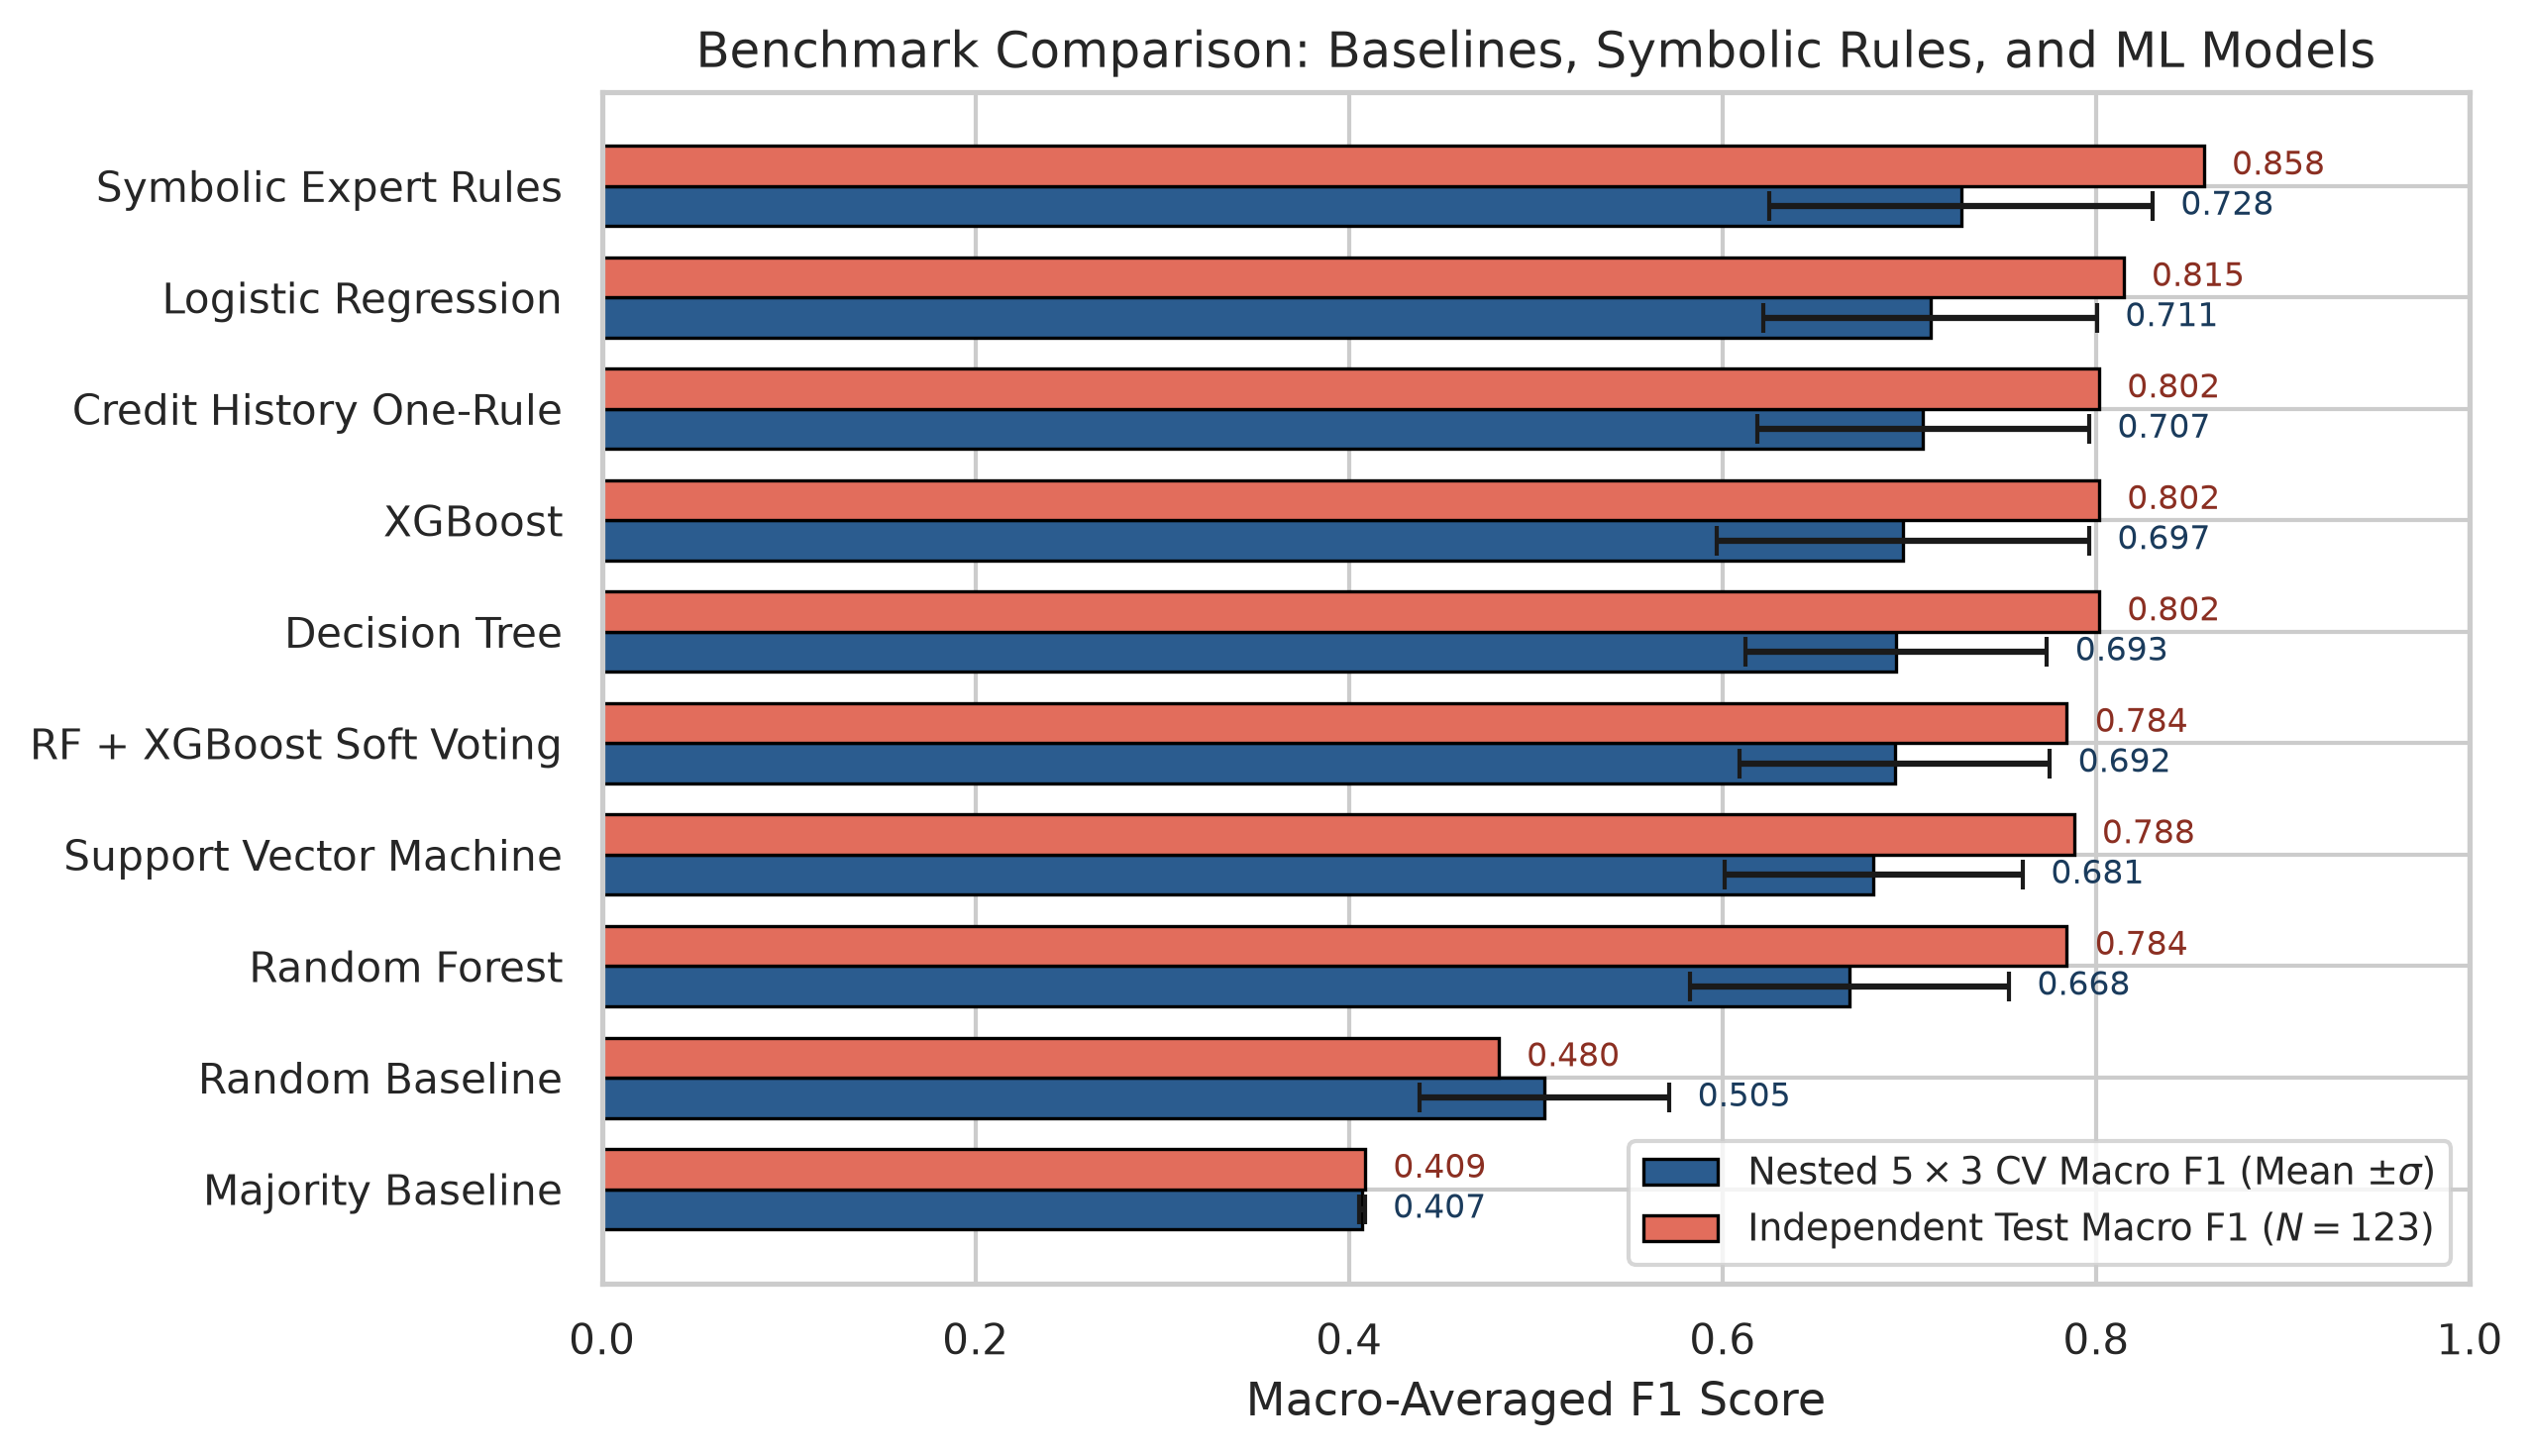
\includegraphics[width=\columnwidth]{model_comparison.png}
\caption{Nested $5\times 3$ CV Macro F1 ($\mu \pm \sigma$) versus held-out test Macro F1 ($N=123$) across all ten evaluated models.}
\label{fig:model_comparison}
\end{figure}

\begin{figure}[t]
\centering
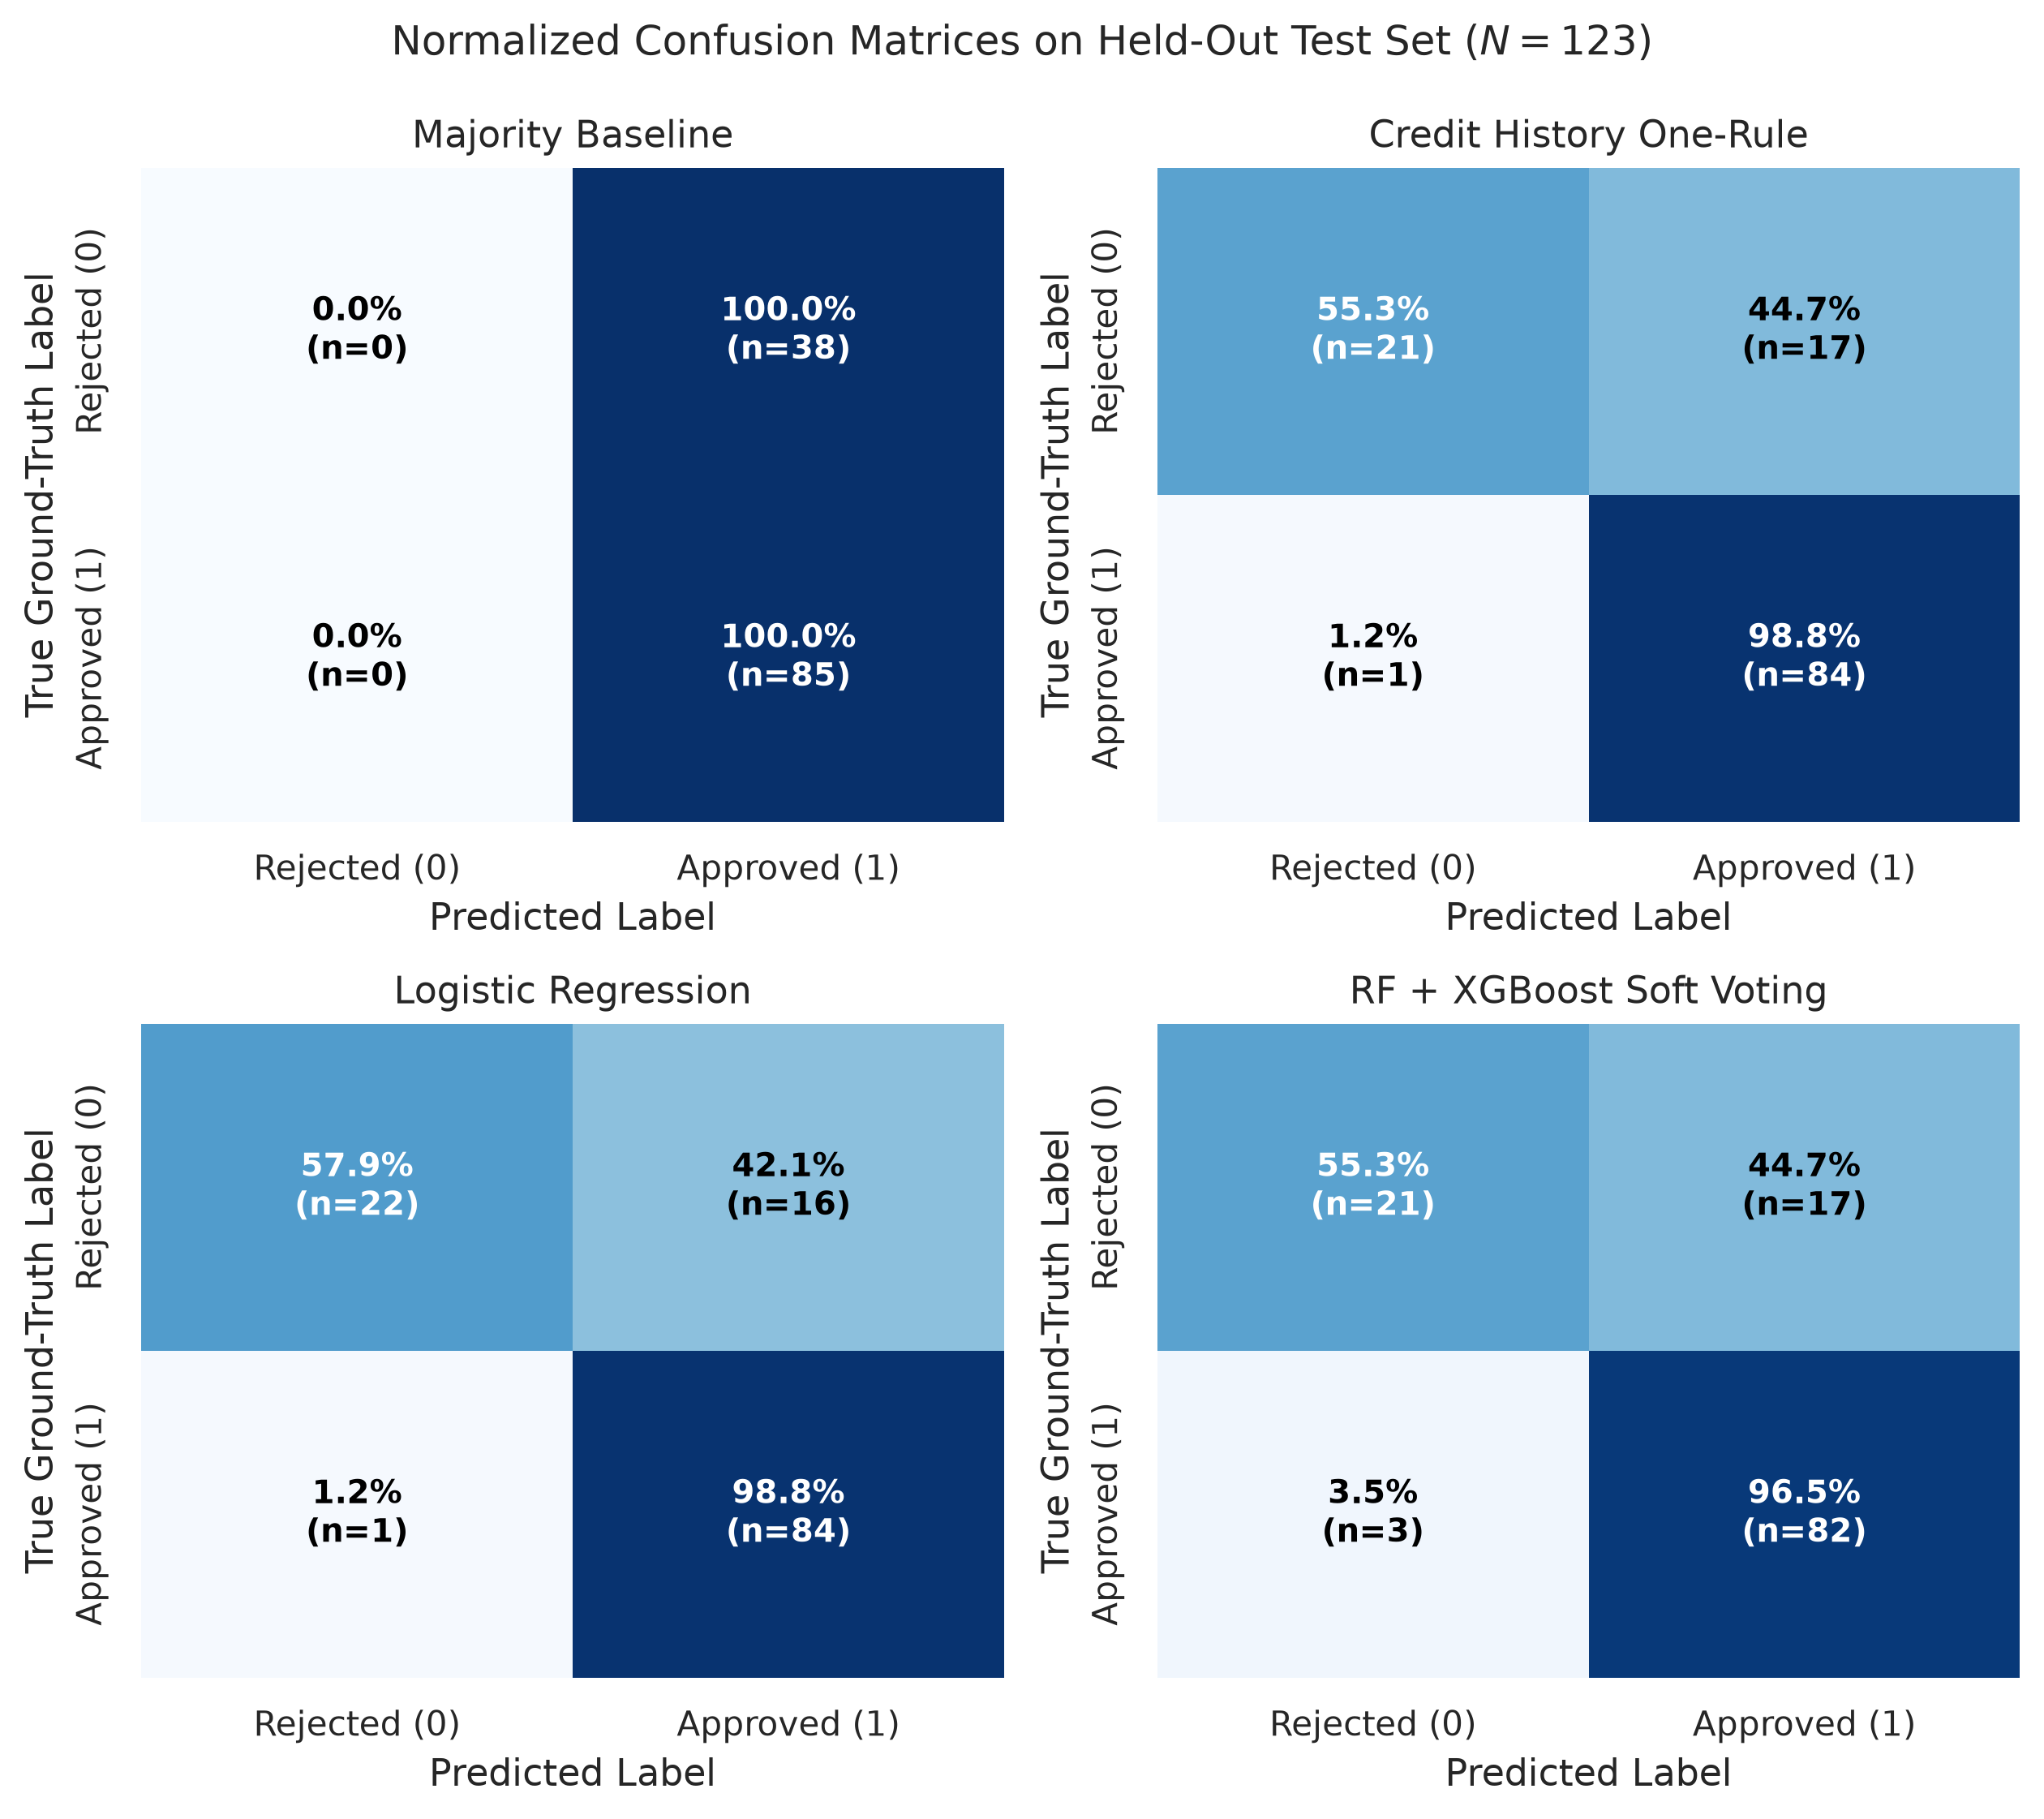
\includegraphics[width=\columnwidth]{confusion_matrices.png}
\caption{Normalized test confusion matrices ($N=123$). Adding the LTI affordability rule raises rejection recall from $55.3\%$ to $71.1\%$, cutting false approvals from 17 to 11.}
\label{fig:cm}
\end{figure}

\subsection{Comparison with Anchor Study (Gawande et al., 2026)}
Gawande et al.~\cite{gawande2026} evaluate an RF--XGBoost soft-voting ensemble on an expanded $13{,}508$-record, $13$-feature Kaggle loan dataset, reporting \textbf{95.16\% accuracy} and \textbf{0.92 F1-score} on an 80:20 split ($0.948 \pm 0.011$ under 10-fold CV) and outperforming standalone baselines by 4--13 percentage points. On the original $614$-record, $11$-feature dataset, our adapted RF--XGBoost ensemble attains \textbf{83.7\% test accuracy} ($0.784$ Macro F1; nested CV accuracy $0.784 \pm 0.049$)---an $11.4$ percentage-point accuracy gap---and trails both Logistic Regression and symbolic rules.

Three structural factors explain this divergence: (i) \textbf{Sample-size scaling:} $22\times$ fewer training rows ($491$ vs.\ $\approx 10{,}806$) leave tree ensembles unable to stably estimate multi-way interactions (such as \texttt{LoanAmount}--\texttt{ApplicantIncome} reported by Gawande et al.); (ii) \textbf{Feature richness and noise:} the $614$-row corpus contains two fewer predictors and greater unobserved variance among applicants with positive credit history (where rejection occurs for institutional reasons outside the recorded variables); and (iii) \textbf{Validation rigor:} nested $5\times 3$ CV eliminates hyperparameter selection optimism that inflates non-nested benchmarks. Thus, ensemble superiority in retail lending is strongly regime-dependent rather than universal~\cite{dumitrescu2022,chen2024}.

\section{Critical Discussion and Review}
\label{sec:discussion}

\subsection{Emergence of AI and Asymmetric Cost Tuning (LO1, LO2)}
Credit scoring has progressed from judgmental underwriting to linear scorecards and gradient-boosted ensembles~\cite{lessmann2015}. Yet tabular financial models remain bounded by predictor signal and must reflect asymmetric business loss~\cite{hand2009}:
\begin{equation}
\mathcal{C}(\tau) = C_{\text{FP}} \cdot \text{FP}(\tau) + C_{\text{FN}} \cdot \text{FN}(\tau), \quad C_{\text{FP}} = 5.0, \; C_{\text{FN}} = 1.0
\end{equation}
To preserve strict leak-free evaluation, we select $\tau^*$ exclusively on the ensemble's training OOF probabilities ($N=491$) and evaluate the frozen threshold once on the held-out test set ($N=123$) (Figure~\ref{fig:cost_tradeoff}). Training OOF optimization selects $\tau^* = 0.84$, reducing OOF penalty from $482.0$ ($98.2$/100 apps) to $317.0$ ($64.6$/100 apps; $-34.2\%$). Applied untouched to the test set, $\tau^*=0.84$ lowers portfolio loss from $88.0$ ($\text{FP}=17, \text{FN}=3$) at $\tau=0.50$ to $83.0$ ($\text{FP}=4, \text{FN}=63$)---a genuine \textbf{5.7\% out-of-sample loss reduction}. Crucially, while $\tau^*=0.84$ slashes costly false approvals by $76.5\%$ ($17 \to 4$), it sharply increases rejected good borrowers ($3 \to 63$), highlighting both the calibration sensitivity of small-sample probabilities and how test-set threshold tuning would overstate savings.

\begin{figure}[t]
\centering
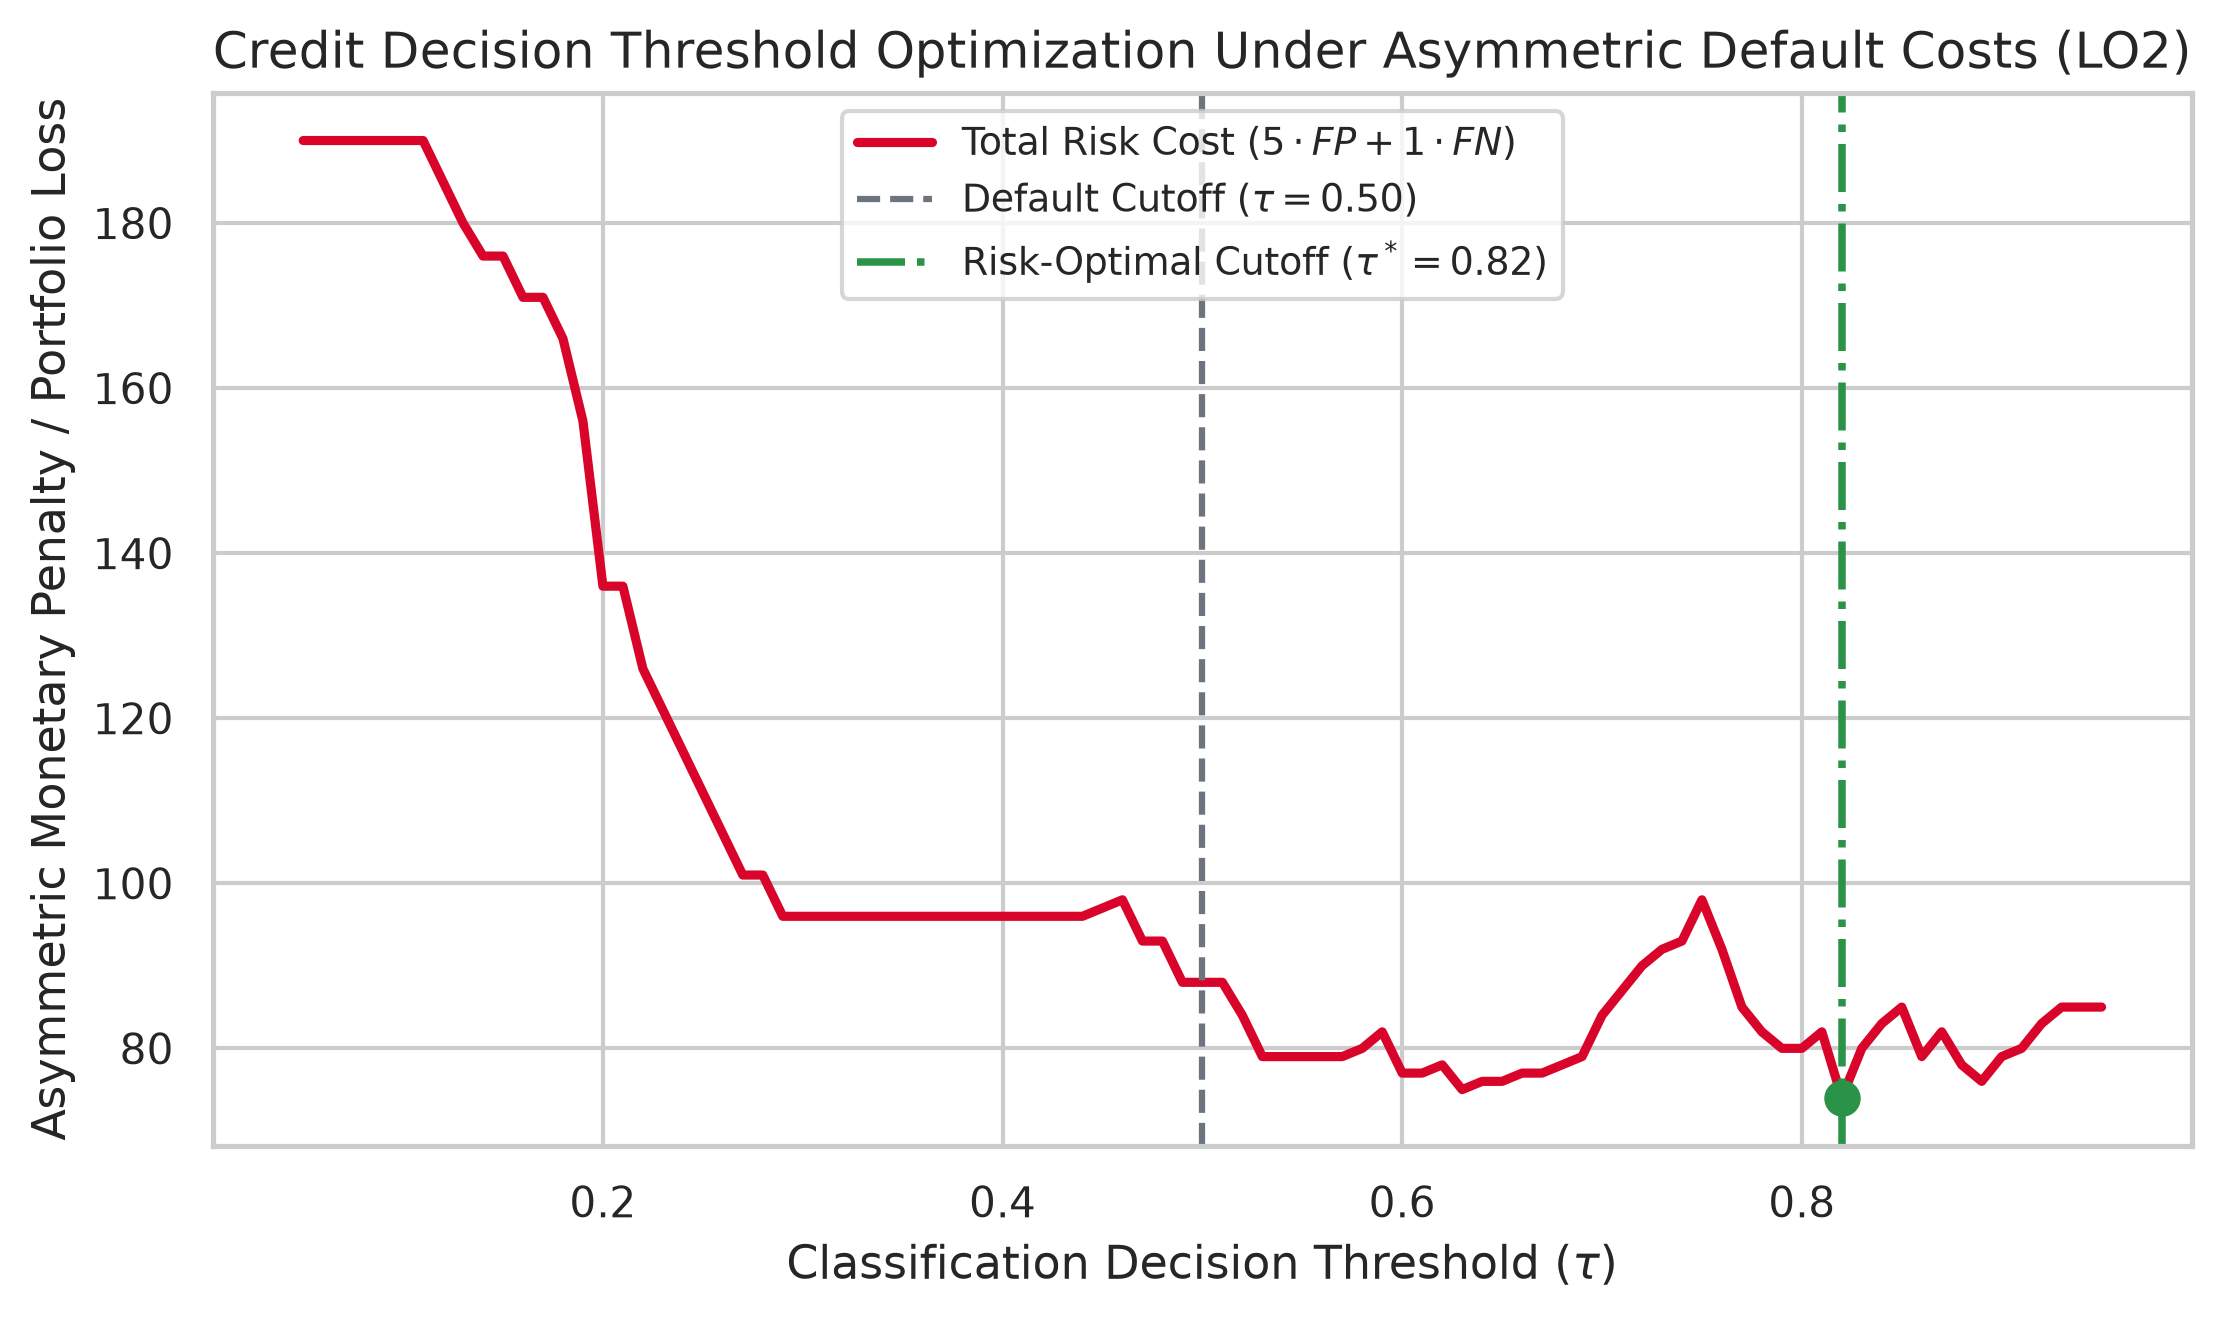
\includegraphics[width=\columnwidth]{calibration_cost_tradeoff.png}
\caption{Leak-free asymmetric cost tuning ($5\cdot\text{FP}+1\cdot\text{FN}$ per 100 applications). Cutoff $\tau^*=0.84$ is selected strictly on training OOF probabilities and verified on held-out test data (LO2).}
\label{fig:cost_tradeoff}
\end{figure}

\subsection{Symbolic AI vs.\ Statistical Machine Learning (LO3)}
Our results directly speak to the symbolic-versus-statistical debate~\cite{rudin2019,bussmann2021}:
\begin{itemize}
    \item \textbf{Symbolic Expert Systems:} Encoding domain structure (credit history plus the $3.0\times$ LTI ratio) injects strong prior knowledge that ML models struggle to rediscover from $491$ rows, yielding our highest Macro F1 ($0.858$ test; $0.728$ CV) alongside deterministic GDPR Article 22 and FCRA adverse-action traceability. Their weakness is rigidity when macroeconomic regimes or nonlinear multi-attribute interactions shift.
    \item \textbf{Statistical ML \& Ensembles:} Logistic Regression and tree ensembles adapt automatically as sample sizes grow (as in Gawande et al.~\cite{gawande2026}) and output continuous risk scores for threshold calibration, but require post-hoc XAI and risk overfitting small datasets.
    \item \textbf{Hybrid Recommendation:} Production lending should pair transparent symbolic policy gates (hard eligibility and affordability caps) with calibrated statistical scoring for borderline applicants~\cite{dumitrescu2022}.
\end{itemize}

\begin{figure}[t]
\centering
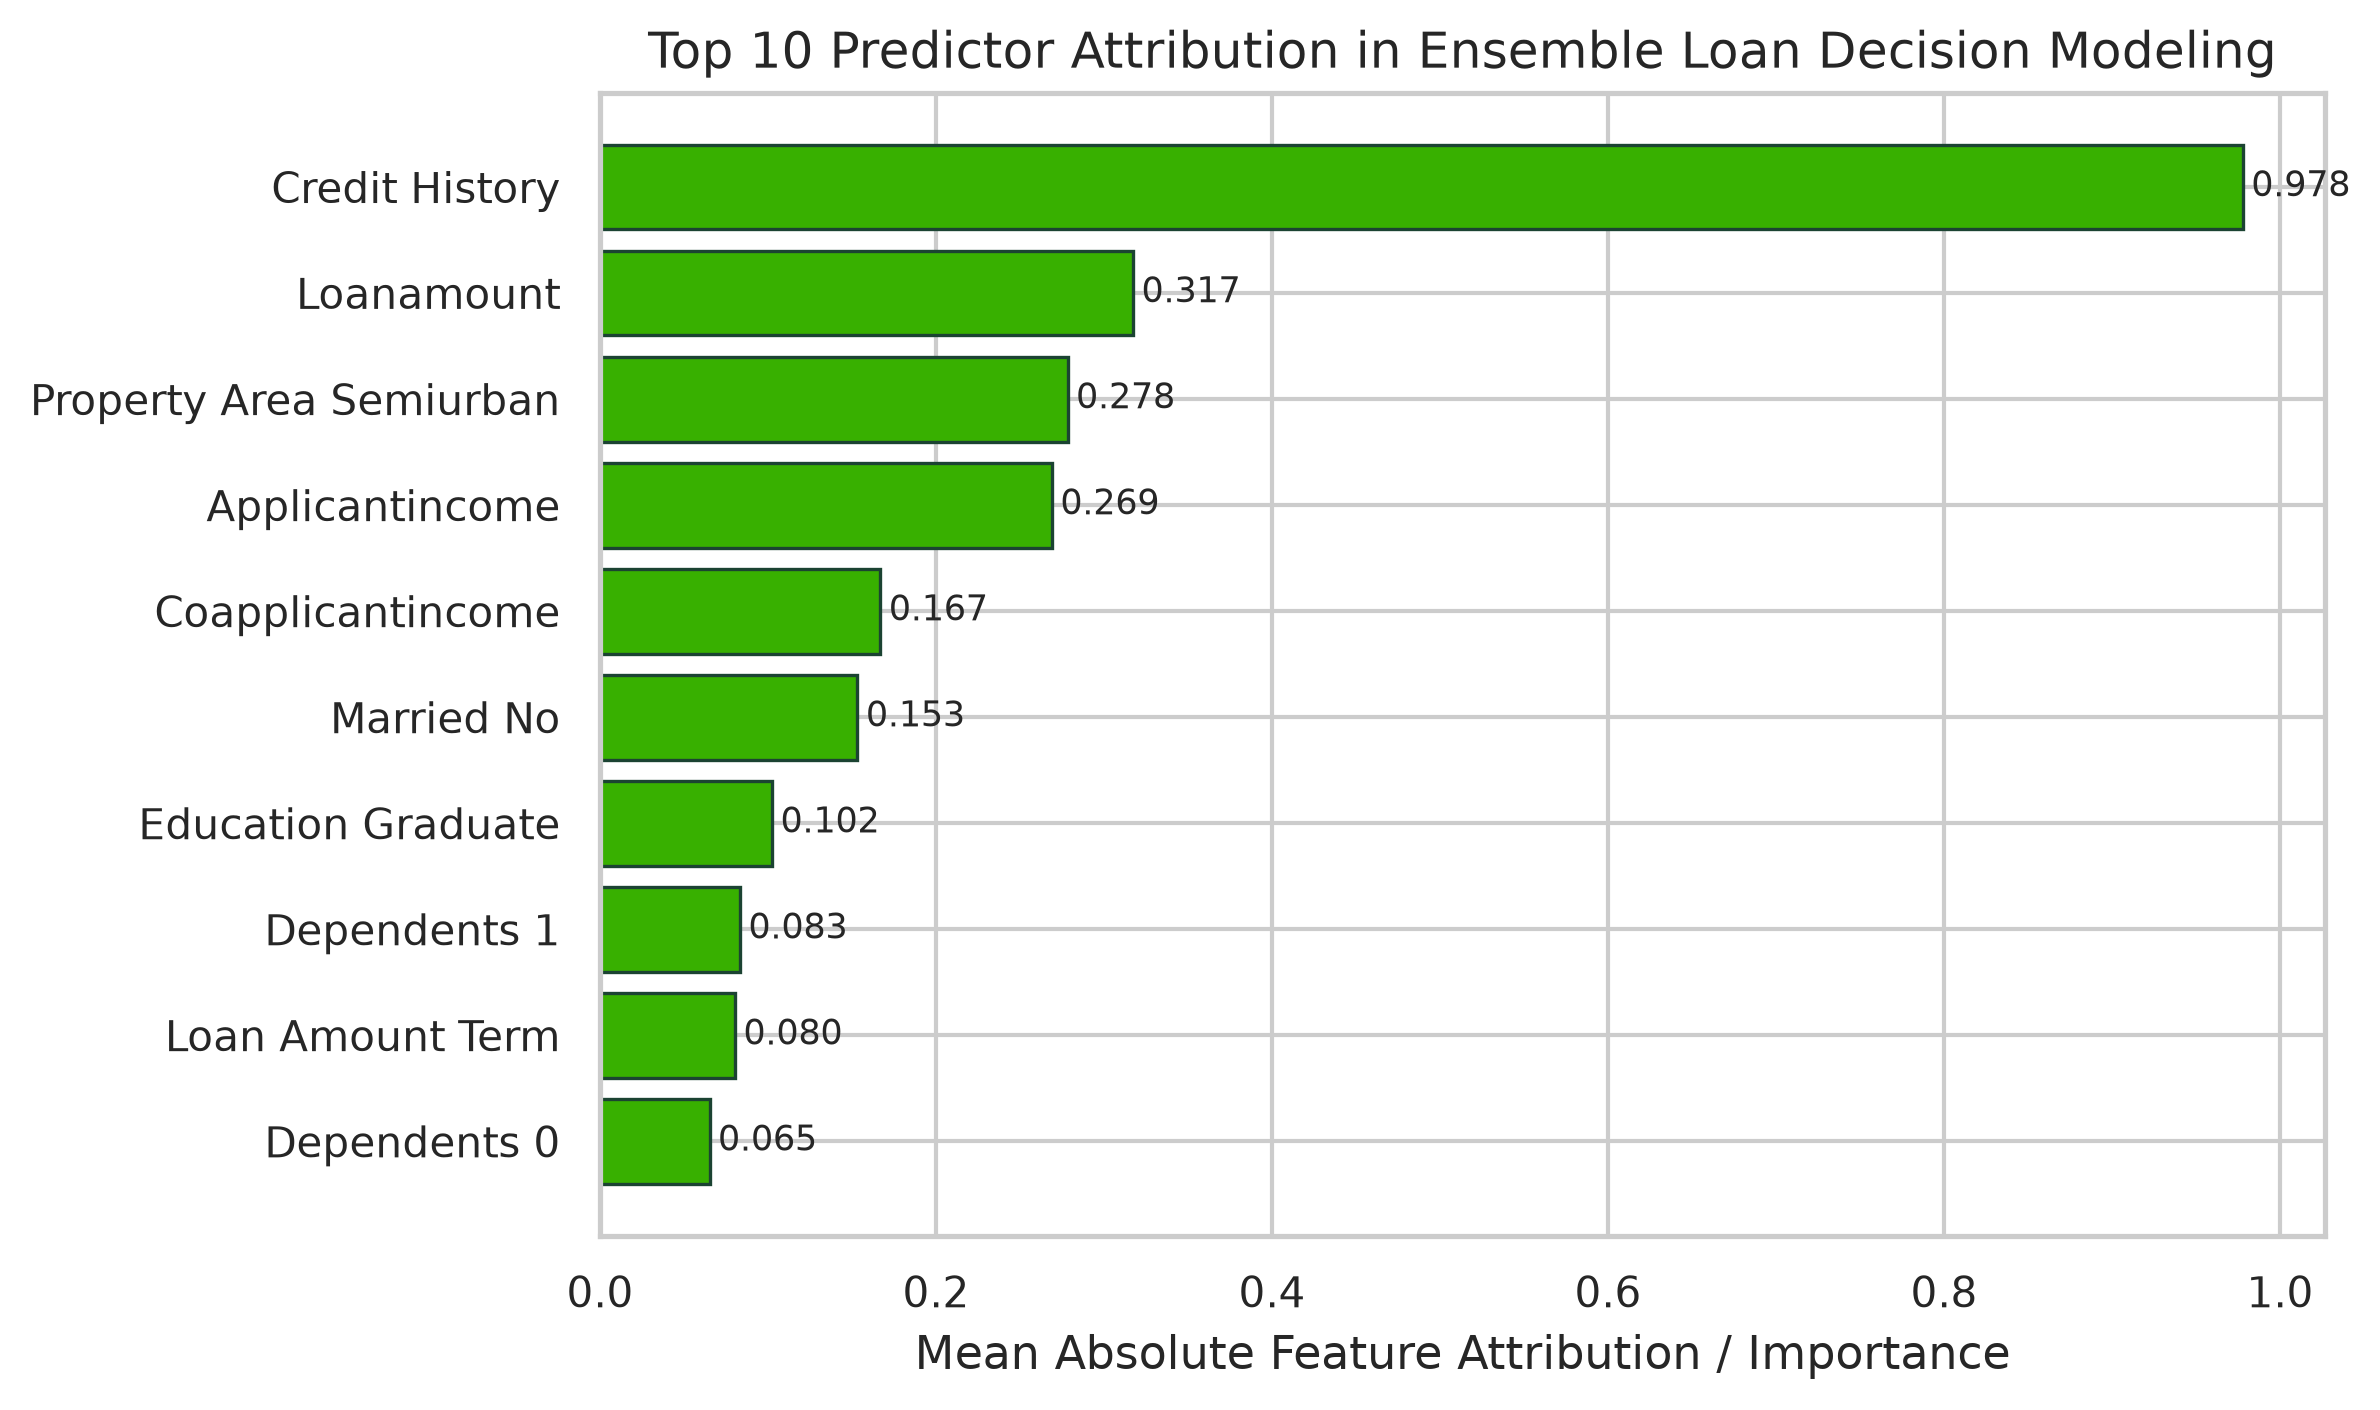
\includegraphics[width=\columnwidth]{feature_importance.png}
\caption{Full-ensemble explainability for RF + XGBoost Soft Voting: (a) exact probability-space weighted TreeSHAP; (b) model-agnostic permutation importance (30 repeats, Macro F1 drop).}
\label{fig:shap}
\end{figure}

\subsection{Ensemble Explainability, Fairness, and Limitations}
By linearity of Shapley values~\cite{lundberg2017}, we compute exact probability-space SHAP values across the full soft-voting ensemble ($\phi^{\text{ens}} = \frac{2}{3}\phi^{\text{rf}} + \frac{1}{3}\phi^{\text{xgb}}$) alongside 30-repeat permutation importance on raw features (Figure~\ref{fig:shap}). \texttt{Credit\_History} dominates both diagnostics, contributing mean $|\phi|=0.134$ ($41.5\%$ of total ensemble probability attribution) and a $0.298 \pm 0.046$ Macro F1 permutation drop, while \texttt{LoanAmount} ($0.030$, $9.2\%$) and \texttt{Property\_Area\_Semiurban} ($0.029$, $9.1\%$) exert smaller probability shifts with near-zero hard-classification permutation impact. Heavy dependence on historical credit flags risks perpetuating exclusion of ``thin-file'' applicants, and demographic proxies (\texttt{Married}, \texttt{Property\_Area}) warrant ongoing fairness auditing~\cite{lin2026,bueff2022}. Moreover, the Kaggle target captures historical lending decisions rather than realized post-disbursement defaults.

\section{Conclusion}
\label{sec:conclusion}
Adapting Gawande et al.~\cite{gawande2026} to the canonical $614$-record loan dataset under leak-free nested $5\times 3$ CV shows that ensemble complexity does not guarantee small-sample gains: Symbolic Expert Rules incorporating a $3.0\times$ LTI affordability ceiling achieve the top Test Macro F1 ($0.858$, CV $=0.728 \pm 0.103$), outperforming Logistic Regression ($0.815$) and RF--XGBoost Soft Voting ($0.784$). Exact ensemble SHAP and permutation analyses confirm credit history dominance ($41.5\%$ share; $0.298$ F1 drop), while leak-free OOF threshold tuning ($\tau^*=0.84$) achieves a verified $5.7\%$ out-of-sample risk-cost reduction. Rigorous baselines, domain knowledge, and honest validation remain essential in high-stakes financial AI.

\section*{AI Usage Declaration}
In accordance with University of Greenwich assessment regulations, generative AI tools (Google Gemini and OpenAI ChatGPT) were used during project preparation strictly as learning and comprehension aids. Specifically, tools supported preliminary literature searches, clarification of banking regulation terminology (Basel II/III and FCRA adverse-action rules), feedback on modular pipeline structure, and language polishing of LaTeX draft prose. AI was not used to generate substantive experimental outcomes or bypass student problem-solving. The student formulated the experimental methodology, executed and verified all Python scripts and numerical tables, checked all cited DOIs against primary sources, and reviewed, edited, and takes full academic responsibility for all analysis presented in this report.

\bibliography{references_AI}

\end{document}
